\documentclass{beamer}
\usepackage[utf8]{inputenc}
\usepackage{graphicx}

\hypersetup{
    colorlinks,%
    citecolor=blue,%
    filecolor=blue,%
    linkcolor=blue,%
    urlcolor=blue 
    %urlcolor=mygreylink     % can put red here to better visualize the links
}

\author[Sowmya Vajjala]{Instructor: Sowmya Vajjala}

\title[LING 520]{LING 520: Computational Analysis of English}
\subtitle{Semester: FALL '16}

\date{1 November 2016}

\institute{Iowa State University, USA}
%%%%%%%%%%%%%%%%%%%%%%%%%%%

\begin{document}

\begin{frame}\titlepage
\end{frame}

\begin{frame}
\frametitle{Class Outline}
\begin{itemize}
\item Exercise from Thursday %15
\item Assignment 4 Discussion %15
\item Overview of constituency parsing methods %30
\item very briefly about Dependency Parsing %15
\item Assignment 5 Description %5
\end{itemize}
%Thursday: Partial parsing, NLTK practice of parsing. Usage of stanford parser.
\end{frame}

\begin{frame}
\frametitle{Exercise from Thursday}
\framesubtitle{Source: Chapter 8 in NLTK Book}
\begin{enumerate}
\item Follow the groucho grammar example in Section 1.2 and simple grammar example in Section 3.1 that uses recursive descent parser.
\item After that, use the grammar in Section 3.3 instead of groucho grammar, and try to parse examples 10 (a) and (b) in the textbook with this grammar.
\item Finally: Figure out how to make Example 3.2 work on your computer, with your own custom created grammar.
\end{enumerate}
- Did everyone finish this?. \pause Sonca is going to come and talk about this exercise now.  
\end{frame}

\begin{frame}
\frametitle{Assignment 4 Discussion}
\begin{itemize}
\item Q1 of A3 and A4: I will have a inclass discussion about them when we discuss NLP4CALL soon.
\item A4-Q2: Stephanie agreed to talk about her writeup. 
\end{itemize}
\end{frame}

\begin{frame}
\frametitle{Parsing Fun}
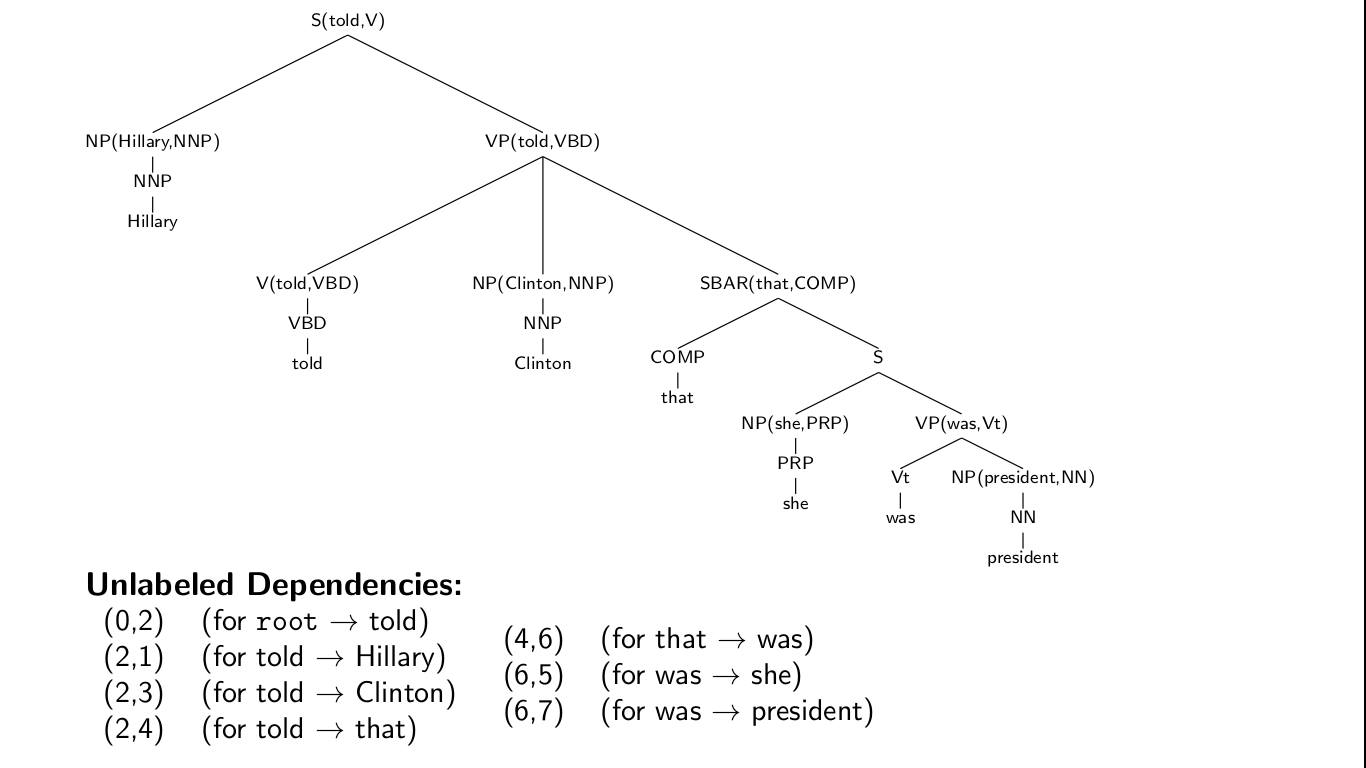
\includegraphics[width=\textwidth]{collinsparse.jpg}
\\ Source: Coursera course by Michael Collins, from 2013 or early 2014. 
\end{frame}

\begin{frame}
\frametitle{}
\Large Constituent Parsing Methods
\end{frame}

\begin{frame}
\frametitle{Constituent Parsing Methods}
 Broadly speaking, there are two ways of doing constituent parsing:
\begin{itemize}
\item Top-down parsing: Start from the root of the parse tree, and go towards the end when you reach the words of the sentence.
\item Bottom-up parsing: Start from the words in the sentence, and go upwards building the parse tree. 
\end{itemize}
All phrase structure parsers use one of these strategies in their parsing algorithms (or a combination of both)
\end{frame}

\begin{frame}
\frametitle{Top-Down parsing}
\begin{itemize}
\item Start with the rule that has the Sentence (S) or ROOT (depending on how your grammar is written) as parent.
\item Look at all grammar rules that has a S on LHS. Mark all of them as a possibility.
\item Explore each rule, recursively keep going further and further down until you see a leaf node.
\item If the rule appears incompatible anywhere, backtrack to previous step and keep doing this until you reach the end of a sentence.
\item Top-down parsing uses grammar to predict the input sentence structure, but without inspecting the input first!!
\end{itemize}
\end{frame}

\begin{frame}
\frametitle{Recursive Descent parsing}
\begin{itemize}
\item Recursive Descent parser is a form of top-down parser.
\item nltk.app.rdparser() has a good demo of how this works. \pause
\item Advantage: Finds all possible correct parses.
\item Disadvantage: This kind of approach to parsing has 3 major short comings.
\begin{enumerate}
\item Left-recursive rules (e.g., NP $->$ NP PP) will make this parser fall in an infinite loop. \\ 
(Example: Edit the parser app to add this rule and see what happens).
\item This parser wastes a lot of processor resources trying to explore paths that are unrelated to the sentence being parsed.
\item While back-tracking, it starts rebuilding all discarded constituents again.
\end{enumerate}
\item One alternative: Do Bottom-up Parsing 
\end{itemize}
\end{frame}

\begin{frame}
\frametitle{Bottom-up parsing}
\begin{itemize}
\item Idea: Start from the sentence, build the tree bottom up, finally reaching the root node.
\item Example: Shift-Reduce parser in NLTK - nltk.app.srparser() \pause
\item Advantage: This works only with rules that match actual words in the sentence. So, does not explore irrelevant options.
\item Disadvantage: May not find a right parse even if there is one. 
\item What to do?: Combine both approaches (LeftCornerParser in NLTK)
\end{itemize}
\end{frame}

\begin{frame}
\frametitle{Dynamic Programming for Parsing}
\begin{itemize}
\item For ambiguous, and long sentences, both top-down and bottom-up approaches become very inefficient because of the number of possible parse paths to explore
\item Dynamic programming helps solve this problem by storing all partial parses generated during the parsing process in a "chart". 
\item This avoids the re-parsing problem of seen parses, and the partially solves ambiguity issues as well.
\item Three commonly used parsers of this kind: chart parser, earley parser, CKY parser
\item Note: Chart parsers can be top-down or bottom-up. \pause
\item Real word parsing: Stanford parser uses an implementation of CKY (bottom-up) parsing with probabilistic grammar.
\item More on the exact algorithms: Chapter 13.1--13.4 in J\&M. 
\end{itemize}
\end{frame}

\begin{frame}
\frametitle{Constituency Parsing in NLTK}
\begin{itemize}
\item NLTK has several parsing algorithms implemented in Python. Some Top-down, some bottom-up, some hybrid \\ (\url{http://www.nltk.org/howto/parse.html})
 \pause
\item If you are really curious about the differences between different parsers in NLTK, visit this: \url{https://goo.gl/9dgGlq}
\item All these examples expect you to provide a grammar. You can also create a grammar out of treebank data in NLTK (Section 6 in Chapter 8 of NLTK book). 
\item My suggestion: NLTK has interface code written to interact with external parsers such as Stanford parser - better use these for real-world use.
\item Note: Parsing is a very active are of R\&D, and there are full courses focusing on Parsing algorithms alone, around the world.
\end{itemize}
\end{frame}

\begin{frame}
\frametitle{}
\Large Dependency Parsing
\end{frame}

\begin{frame}
\frametitle{Dependency Parsing: Methods}
\begin{itemize}
\item What you need: a set of dependency relations, lexicon of the language.
\item You can again do top-down, bottom-up, a combo, use Dynamic programming etc.
\item Not as much explored as constituency parsing in NLP.
\item Malt parser: a state-of-the-art dependency parser that uses dynamic programming with bottom-up parsing.
\item Stanford dependency parser: This is not primarily a dependency parser, it converts constituency tree into dependency relations.
\item Dependency relations encode relations between words. So useful for information extraction.
\end{itemize}
\end{frame}

\begin{frame}
\frametitle{Dependency Parsers in NLTK}
\begin{itemize}
\item NLTK does not have a real dependency parser. But it has interface code to existing dependency parsers such as MALT parser and Stanford Dependency parser.
\item spacy.io has support for Dependency parsing in Python. If you want, figure out its installation and use that!
\item MATE parser is another popular dependency parser (works for English and German).
\end{itemize}
\end{frame}

\begin{frame}
\frametitle{Dependency Parsing and CALL}
\begin{itemize}
\item Dependency parsing is relatively tolerant to word-order changes. So, it is used by NLP-CALL researchers to analyse the syntactic structure of learner language more commonly than constituency parsing.
\item Parsing learner language is an active area of research in NLP researchers who work in CALL topics.
\item Will discuss briefly about this in a few weeks
\end{itemize}
\end{frame}

\begin{frame}
\frametitle{}
\Large Assignment 5 Description
\end{frame}

\begin{frame}
\frametitle{Next Class}
\begin{enumerate}
\item Topics: 
\begin{itemize}
\item Partial Parsing, incremental parsing and other such methods
\item Parsing: Conclusion
\item practice exercises with using parsers in Python
\end{itemize}
\item Readings: Chapter 8 in NLTK (Mandatory). Chapter 12--14 in J\&M (Optional)
\item Video lectures (optional): Week 5 Lectures in Jurafsky and Manning's course or Weeks 4 and 5 lectures in Radev's course.
\end{enumerate}
\end{frame}

\begin{frame}
\frametitle{If there is time: another Exercise}
Figure out how to use Stanford parser in Python (with or without NLTK). I will ask about this in Thursday's class. 
\end{frame}

\end{document}

%
%Parsing practice: http://coling.epfl.ch/TP/Parsing.html

%For NLP-CALL interface class on 15th Nov:
http://urd.let.rug.nl/nerbonne/papers/nlp-hndbk-call.pdf
Meurers-11: http://tjure.sfs.uni-tuebingen.de/~dm/papers/meurers-11.pdf
The promise of NLP and speech processing technologies in language assessment (http://ltj.sagepub.com/content/27/3/301.abstract)
Towards Adaptive CALL: Natural Language Processing (NLP) for Diagnostic Language Assessment
(https://apling.engl.iastate.edu/alt-content/uploads/2015/05/5thTSLL2007_proceedings.pdf)
Parsing for CALL: PST or Dependency - which can handle grammatical errors better?
%Where I am coming from: BEA; NLP4CALL;
%Other related satellite events.
%overview of tasks etc.

%17th: Assignment 5 discussion, bonus points details, Problem Set 8 exercises, NLP4CALL-details on what you need to know.	

\begin{frame}
\frametitle{Programming exercise - 1}
\begin{itemize}
\item Take any .txt version file from gutenberg.org, written by your favorite author (in English!)
\item Read that file into your python code, and do the following using NLTK:
\begin{enumerate}
\item Split the file into sentences.
\item Print the following: number of sentences in the file, average sentence length (in number of words), average word length (in number of characters), number of unique words, number of unique stems.
\item Note 1: Once sentence splitting is done, you can ignore punctuation markers for the rest of the calculation.
\item Note 2: You can use any stemmer you want.
\end{enumerate}
\end{itemize}
\end{frame}

\begin{frame}
\frametitle{Programming exercise - 1}
\begin{itemize}
\item For the same file from last slide, do the following:
\item Read that file into your python code, and do the following using NLTK:
\begin{enumerate}
\item Split the file into sentences.
\item For each sentence, print its POS tagged version as a string of tags. E.g., if you have "It is a sentence" as your sentence, and your NLTK tagger outputs the tags for this sentence as a list (or tuple or whatever), you should print the tag as a string. E.g., PRP VBZ DT NN (not as [PRP, VBZ, DT, NN] or as [(It, PRP), (is, VBZ) .. ... ])
\end{enumerate}
\end{itemize}
\end{frame}
